\documentclass[11pt,a4paper]{article}

% Package imports
\usepackage[utf8]{inputenc}
\usepackage[T1]{fontenc}
\usepackage{lmodern}
\usepackage{graphicx} % For including images
\usepackage{geometry}
\usepackage{xcolor}
\usepackage{tcolorbox}
\usepackage{titlesec}
\usepackage{hyperref}
\usepackage{enumitem}
\usepackage{fancyhdr}
\usepackage{tikz}     % For positioning and layering
\usetikzlibrary{arrows.meta}
\usetikzlibrary{graphs, positioning}

% Page layout
\geometry{top=0.8in, bottom=0.6in, left=0.8in, right=0.8in}
\setlength{\parindent}{0em}
\setlength{\parskip}{0.5em}

% Colors
\definecolor{primary}{HTML}{23373B}
\definecolor{secondary}{HTML}{38774D}
\definecolor{accent}{HTML}{E74C3C}
\definecolor{bg}{HTML}{ECF0F1}

% Hyperlinks
\hypersetup{
    colorlinks=true,
    linkcolor=secondary,
    urlcolor=accent,
    citecolor=secondary
}

% Title formatting
\titleformat{\section}{\normalfont\LARGE\bfseries\color{primary}}{\thesection}{1em}{}
\titleformat{\subsection}{\normalfont\Large\bfseries\color{secondary}}{\thesubsection}{1em}{}
\titleformat{\subsubsection}{\normalfont\large\bfseries\color{primary!80}}{\thesubsubsection}{1em}{}

% tcolorbox for highlights
\tcbset{
    colframe=secondary,
    colback=bg,
    coltitle=white,
    boxrule=1pt,
    left=0.5em,
    right=0.5em,
    top=0.2em,
    bottom=0.2em
}
\setlist{itemsep=0.2em, topsep=0.2em}

\titlespacing{\section}{0pt}{*0.5}{*0.5}
\titlespacing{\subsection}{0pt}{*0.4}{*0.4}
\titlespacing{\subsubsection}{0pt}{*0.3}{*0.3}

\pagestyle{fancy}

\fancyhf{} % Clear header and footer
\fancyhead[L]{\textbf{\color{primary}Daniel Cermann}} % Left header
\fancyhead[R]{\textbf{\color{primary} January 28, 2025}} % Right header

% Document starts here
\begin{document}

\nocite{*}

\thispagestyle{empty}
% Title
\begin{center}
    {\huge \textbf{\color{primary} Temporal Graphs}} \\
    \vspace{0.4em}
    {\Large \color{secondary} Algorithmic Gems for Graphs, Probabilities and Processes Winter semester 24/25}
    \vspace{1em}
    \rule{\textwidth}{0.5pt}
\end{center}
\section{Motivation}
\begin{minipage}{0.6\textwidth}
\begin{itemize}
  \item Route finding in transportation networks
  \item distributed networks $\rightarrow$ analysis of various properties
  \item dissemination processes
\end{itemize}
\end{minipage}
\begin{minipage}{0.39\textwidth}
  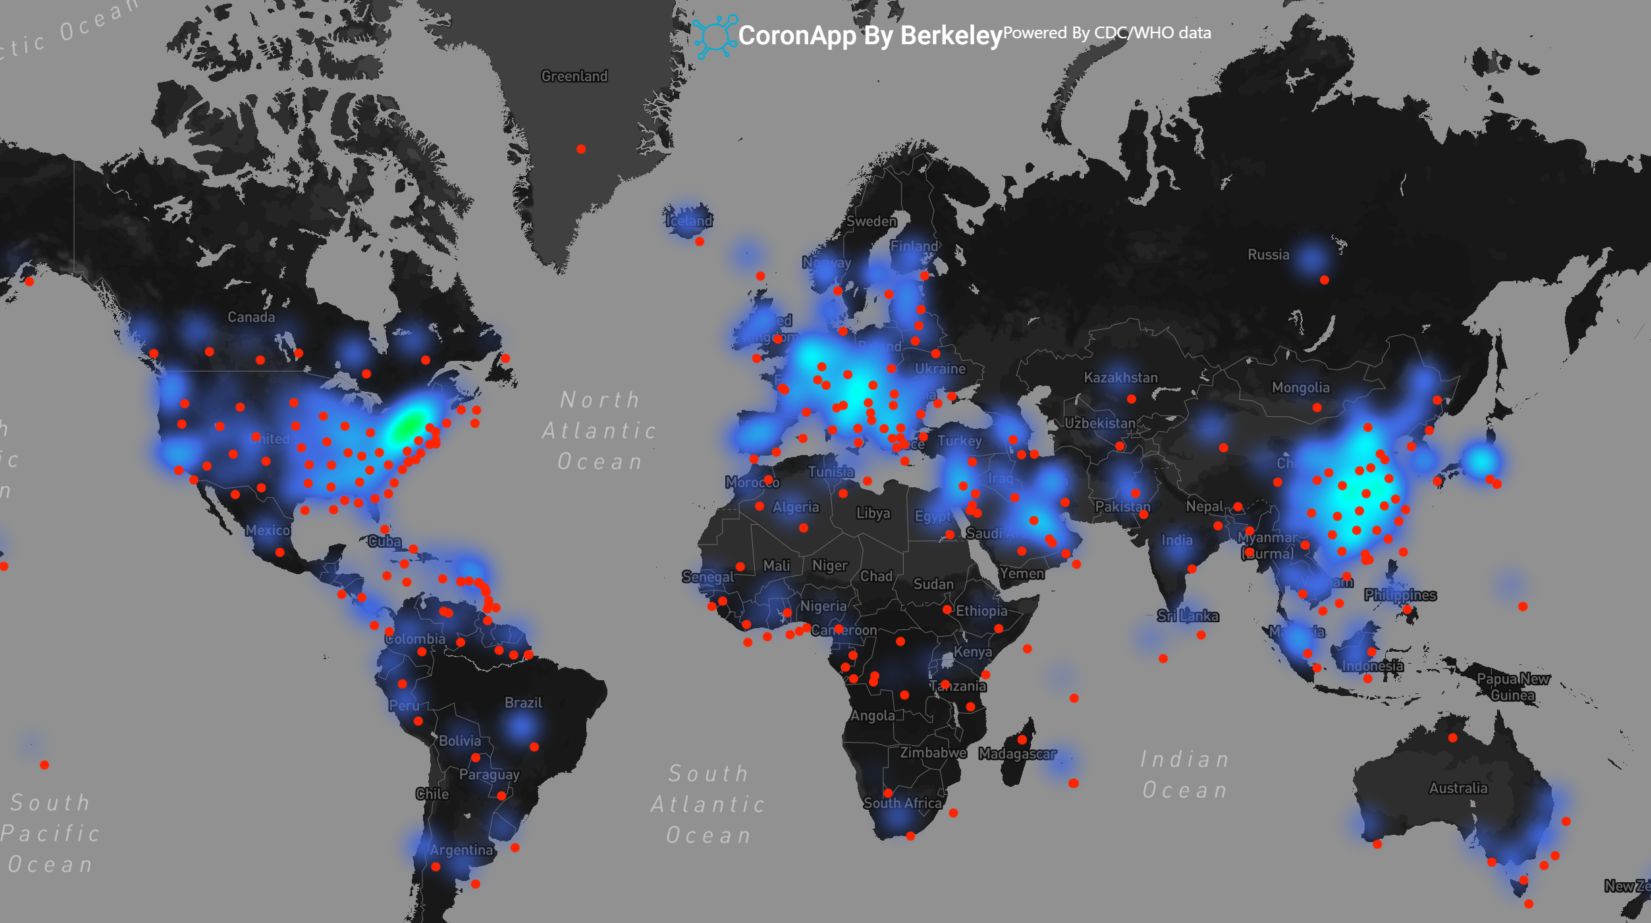
\includegraphics[width=0.9\textwidth]{media/corona.png}
\end{minipage}


\section{Basic terms and definitions}

\begin{tcolorbox}[title=Definition temporal graph]
  A \textbf{temporal graph} \cite[page 243]{Michail2015} is is triple \( G = (V, E, \lambda) \) where:
  \begin{itemize}
        \item \( (V, E) \) is a graph
        \item $ \lambda: E \rightarrow 2^{\mathbb{N}}$ is a mapping of edges to a set natural numbers (time steps when this edge is active)
      \end{itemize}
\end{tcolorbox}

\subsection{Exercise}
\begin{center}
  \scalebox{1.5}{
  \begin{tikzpicture}[
      every node/.style={circle, draw, minimum size=0.3cm, font=\small},
      every edge/.style={draw, ->, font=\tiny},
      labelstyle/.style={draw=none, font=\tiny, midway, maximum size=0.3cm, inner sep=0.1pt},
      >=stealth
  ]
  % Define vertices
  \node (C) at (0, 0) {C};
  \node (H) at (2, 0) {H};
  \node (B) at (4, 0) {B};
  \node (G) at (6, 0) {G};
  \node (W) at (8, 0) {W};
  \node (P) at (5, 3) {P};
  \node (M) at (5, -2) {M};
  \end{tikzpicture}}
\end{center}


\subsection{Notation for convenience $\rightarrow$ \cite[p. 243ff]{Michail2015}  \hfill { \small \color{black} for above temporal graph: }}
\begin{itemize}
	\item $\lambda(G)$ - temporal graph with respect to $G$ 
	\item $\lambda(E)$ - multiset of all labels
	\item $| \lambda | = \sum_{e \in E} | \lambda(e) | $
	\item $ \lambda_{min} = min\{l \in \lambda(E)\} $
	\item $ \lambda_{max} = max\{l \in \lambda(E)\} $
	\item $\alpha(\lambda) = \lambda_{max} - \lambda_{min} + 1$ - lifetime of a temporal graph $\lambda(G)$
\end{itemize}

\begin{tcolorbox}[title=Definition: static expansion of a graph]
  The static expansion of a temporal graph $D = (V, A)$ with $V = \{ u_1, u_2, ..., u_n \}$ is a DAG $H = (S, E)$ with:
  $$ S = \{ u_{ij} | \lambda_{min} - 1 \leq i \leq \lambda_{max}, 1 \leq j \leq n \} $$
  and
  $$ E = \{ (u_{(i - 1)j}, u_{ij'}) | \lambda_{min} \leq i \leq \lambda_{max} \land $$
  $$ 1 \leq j, j' \leq n \land (j = j' \lor (u_j, u_{j'}) \in A(i))) \} $$
\end{tcolorbox}

\begin{center}
  \scalebox{1.5}{
  \begin{tikzpicture}
  \tikzset{every arrow/.append style={arrowhead=1cm}} % Adjust scale as needed
  % Define grid size
  \def\rows{6} % number of rows
  \def\cols{8} % number of columns

  % Create nodes in a grid as small points
  \foreach \i in {1, ..., \rows} {
      \foreach \j in {1, ..., \cols} {
          \node[fill=black, circle, inner sep=1pt] at (\j, -\i) {}; % small points
      }
      \draw[dashed, gray] (0.5, -\i) -- (\cols, -\i); % horizontal grid lines
      \node at(\i, -\rows - 0.5) {\i}; % row numbers
  }
  \node (labelC) at (0, -1) {C};
  \node (labelH) at (0, -2) {H};
  \node (labelB) at (0, -3) {B};
  \node (labelG) at (0, -4) {G};
  \node (labelW) at (0, -5) {W};
  \node (labelP) at (0, -6) {P};
  \end{tikzpicture}}
\end{center}

\section{Journeys}
\begin{tcolorbox}[title=Definition: temporal/time respecting walk]
  A \textbf{temporal} or \textbf{time-respecting walk} $W$ of a temporal graph $D = (V, A)$ is an alternating sequence of of nodes and times $(u_1 , t_1 , u_2 , t_2 , ... , u_{k-1} , t_{k-1} , u_k )$
  where 
  \begin{itemize}
    \item $\forall 1 \leq i \leq k - 1: ((u_i , u_{i+1} ), t_i ) \in A$ and
    \item $1 \leq i \leq k - 2: t_i < t_{i + 1}$ 
  \end{itemize}
\end{tcolorbox}
\begin{itemize}
  \item $t_1$ - departure time
  \item $t_{k - 1}$ arrival time
  \item $t_{k - 1} - t_1 + 1$ - duration/temporal length
\end{itemize}

\begin{tcolorbox}[title=Definition: Journey]
  A \textbf{journey} is a is a temporal walk with pairwise distinct nodes \^{=} a journey of D is a path of the underlying static graph of D that uses
strictly increasing edge-labels.
\end{tcolorbox}

\begin{tcolorbox}[title=Definition: Foremost Journey]
  A u-v journey J is called foremost from time $t \in \mathbb{N}$ if it departs after time t and its arrival time is minimized.
\end{tcolorbox}

\begin{tcolorbox}[title=Definition: Temporal distance]
  The \textbf{temporal distance} from a node $u$ to at time $t$ to a node $v$ is defined as the duration of a foremost journey from $u$ to $v$ that departs at time $t$.
\end{tcolorbox}
\begin{tcolorbox}[title=Definition: Temporal diameter $d$]
  The minimum integer $d$ such that there exists a foremost journey from every node $(u, t) \in V \times \{ 0, 1, ..., \alpha - d \}$  to every node $v \in V$ with duration at most $d$.
\end{tcolorbox}

\section{Dissemination processes}
\begin{itemize}
  \item studies spread of information, rumor, fake news, disease, ...
\end{itemize}
\bold\textit{{Vaccination Problem}}: The vaccination problem involves optimizing the allocation and timing of vaccines to control the spread of infectious diseases.\\
\begin{tcolorbox}[title=Neighbourhood Vacination protocol]
    choose a person at random among all persons that have been involved in at least one contact at time t*, ask her to name someone she met, vaccinate this other person, and repeat until a desired fraction of the vertices are vaccinated
\end{tcolorbox}
\subsection{Exercise}
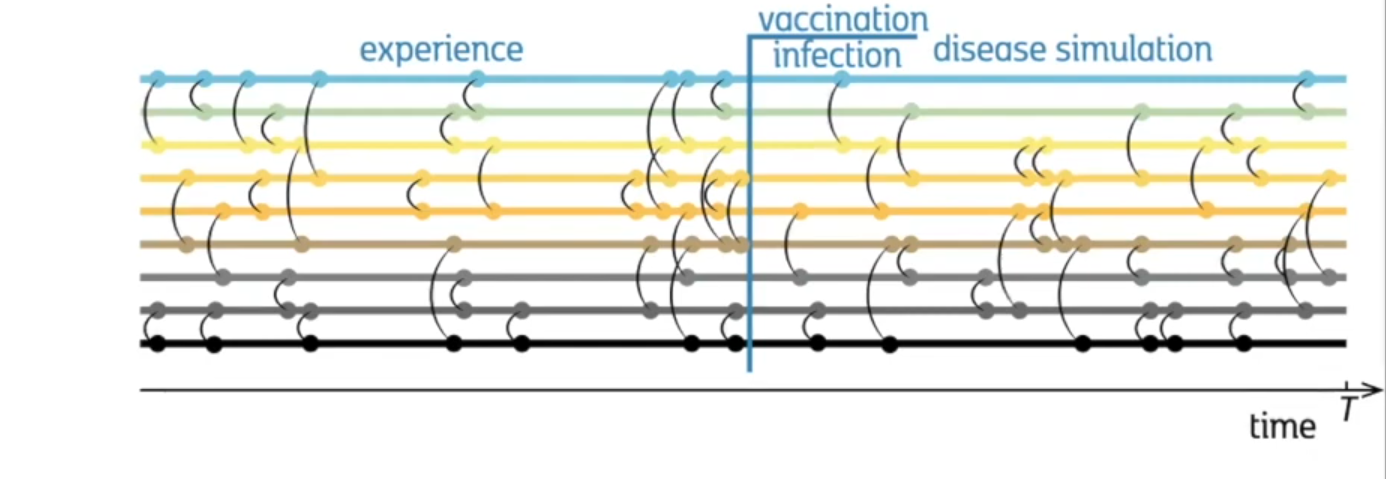
\includegraphics[width=0.9\textwidth]{media/infection_process_a.png}\\
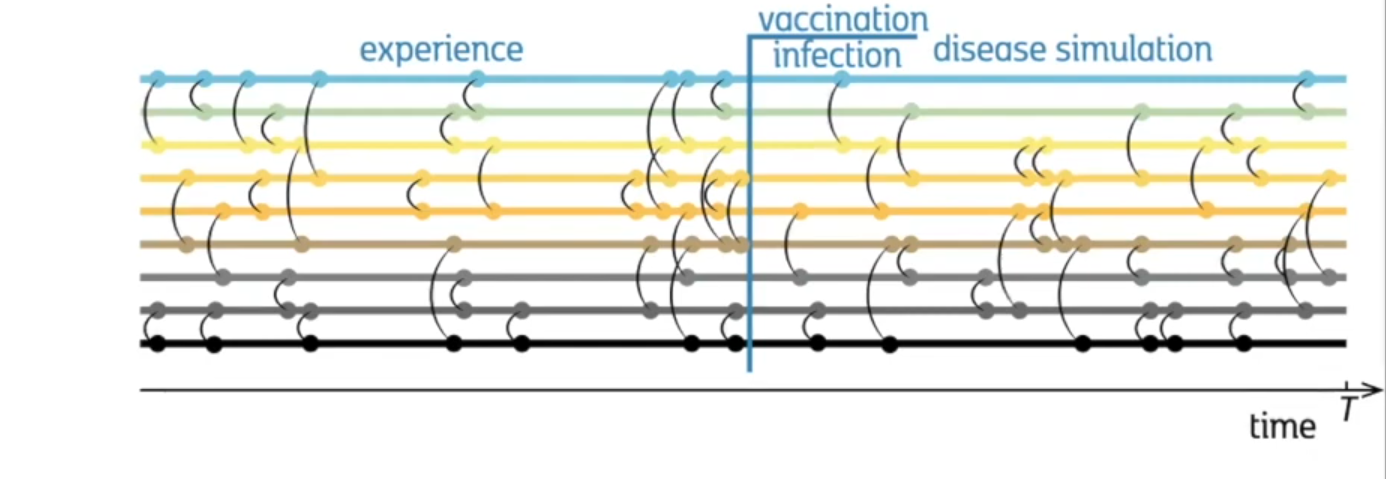
\includegraphics[width=0.9\textwidth]{media/infection_process_a.png}


\newpage

\bibliographystyle{plain} % Choose a bibliography style
\bibliography{references} % Path to your .bib file

\end{document}
